% !TeX spellcheck = en_GB
\documentclass[11pt]{article}

\usepackage[type1]{libertine}
\usepackage[a4paper,top=35mm]{geometry}
\usepackage{parskip}
\usepackage{amsmath, amsthm, amssymb} 
\usepackage{booktabs}
\usepackage{tabularx}
\usepackage[english]{babel}
\usepackage{enumitem}	% remove inline if not needed
\usepackage{gensymb}
\usepackage{bm}
\usepackage{graphicx}
\usepackage{xcolor}
\usepackage{float}
\usepackage{wrapfig}
\usepackage[makeroom]{cancel}
\usepackage{multicol}
\usepackage{multirow}
\usepackage{vwcol} 	 	% Provides variable multicol
\usepackage{commath} 	% Provides good differentials
\usepackage{esint} 		% Provides various fancy integral symbols
\usepackage{siunitx} 	% Provides good units
\usepackage{nicefrac}
\usepackage{dashrule}
%\usepackage{showframe}

\usepackage[titletoc,title,toc,page]{appendix}

\usepackage{hyperref}
\hypersetup{
	pdftitle={SJPO 2018 General Round Suggested Worked Solutions},
	pdfauthor={Sun Yudong, Lor Jun Heng, et al.},
	bookmarksnumbered=true,
	bookmarksopen=true,
	bookmarksopenlevel=2,
	pdfstartview=Fit,
	pdfpagemode=UseOutlines,
	colorlinks=true,
	linkcolor=black,
	filecolor=magenta,      
	urlcolor=blue
}
\urlstyle{same}

% custom environments
\usepackage{tikz}
\newcommand*\circled[1]{\tikz[baseline=(char.base)]{
		\node[shape=circle,draw,inner sep=2pt] (char) {#1};}}

\newcommand{\uvec}[1]{\boldsymbol{\hat{\textbf{#1}}}}
\newcommand{\bvec}[1]{\boldsymbol{\vec{#1}}}
\def\doubleunderline#1{\underline{\underline{#1}}}
\newcommand{\solution}[2]{\textbf{Solution:\hspace{1em}\circled{#1}}\hspace{1em}#2\hspace{1em}}
\newcommand{\calc}{\boxed{\textbf{CALC}} \hspace{1em}}


\renewcommand{\ttdefault}{cmtt}
\newlength{\currentparskip}

\newenvironment{multicolFigure}
{\par\medskip\noindent\minipage{\linewidth}}
{\endminipage\par\medskip}

\title{SJPO 2018 General Round\\Suggested Worked Solutions}
\author{Sun Yudong, Lor Jun Heng\\{\small with contributions from Theodore Yoong}}
\date{June 10, 2018}

\begin{document}
	\maketitle
	The solutions may not be accurate, and serve merely as \textit{suggestions}. Do let us know if you notice any parts that are wrong. This solution set is to be read with the SJPO 2018 General Round Paper, which you should have a copy of. 
	
	Questions labelled with \calc\hspace{-1.1em} require explicit calculus knowledge to solve. 
	
	\begin{enumerate}[label={[Q\arabic*]},itemsep={1em}]
		\item \calc \solution{D}{$\displaystyle f=\frac{1}{2\pi}\sqrt{\frac{2V_0}{\mu\delta^2}}$}
			\vspace{-0.5em}
			\paragraph{Solution 1} \textit{\small provided by Theodore}
			
			The Taylor Expansion of the potential energy function $V(x)$ may be expressed as such:
			\begin{align}
				V(x) &= \left(\cancelto{~\text{constant, can ignore}}{V(x_0)}\right) + \left(\cancelto{0 \text{~at eqm}}{V'(x_0)}\delta x\right) + \left(\frac{V''(x_0)}{2!} \delta x^2\right) + ... \notag \\
				&= \frac{1}{2}V''(x_0)\delta x^2 \equiv \text{Hookean Spring Potential}
			\end{align}
			where $V''(x_0) = k = m\omega^2$. Thus, 
			\begin{equation}
				\omega=\sqrt{\frac{V''(x_0)}{m}}
			\end{equation}
			Now we solve for $V''$:
			\begin{align*}
			V  &= V_0\left[ \left(1-e^\frac{-\left(x-x_0\right)}{\delta}\right)^2-1\right]\\[0.2em]
			V' &= V_0\left[2\left(1-e^\frac{-\left(x-x_0\right)}{\delta}\right)\left(-\frac{1}{\delta}e^{\frac{-\left(x-x_0\right)}{\delta}}\right)\right]\\[0.2em]
			&= \frac{2V_0}{\delta}\left[e^{\frac{-\left(x-x_0\right)}{\delta}}-\frac{1}{\delta}e^{\frac{-2\left(x-x_0\right)}{\delta}}\right] \\[0.2em]
			V'' &=\frac{2V_0}{\delta}\left(-\frac{1}{\delta}e^{\frac{-\left(x-x_0\right)}{\delta}}+\frac{2}{\delta}e^{\frac{-2\left(x-x_0\right)}{\delta}}\right)\\[0.2em]
			V''(x_0)&=\frac{2V_0}{\delta}\left(\frac{1}{\delta}\right)=\frac{2V_0}{\delta^2}
			\end{align*}
			Thus, we obtain:
			\begin{equation}
				f = \frac{\omega}{2\pi} = \doubleunderline{\frac{1}{2\pi}\sqrt{\frac{2V_0}{\mu\delta^2}}}
			\end{equation}
			\vspace{-2em}
			\paragraph{Solution 2} {\small Alternatively, we use the approximation somewhere, and recall that $F=-\dod{V}{r}$}
			
			First, we let $z = \nicefrac{y}{\delta} = \nicefrac{\left(x-x_0\right)}{\delta}$, where $z$ helps us simplify the working, and $y$ is ultimately the variable that determines the force. 
			\begin{align*}
				V(z) &= V_0\left[1-e^{\frac{-\left(\left(\delta z + x_0\right)-x_0\right)}{\delta}}\right]^2-V_0 \\
				&= V_0\left[1-e^{-z}\right]^2-V_0 \\
				&= V_0\left[1+e^{-2z}-2e^{-z}\right]-V_0 \\
				&\approx V_0\left[1+\left(1-2z+\frac{4z^2}{2}\right)-2\left(1-z+\frac{z^2}{2}\right)\right]-V_0\\
				&=V_0\left(z^2\right)-V_0\\
				F(x) =-\dod{V}{y}&=-2V_0z\cdot \dod{z}{y} \\
				&= -2V_0\left(\frac{y}{\delta}\right)\cdot \frac{1}{\delta} \\
				a(x) = \frac{F(x)}{\mu} &= -\frac{2V_0}{\mu\delta^2}y \equiv -\omega^2y
			\end{align*}
			This form tells us that, for a sufficiently small $y$, the molecule undergoes simple harmonic oscillations about the equilibrium position with $\omega^2 = \nicefrac{2V_0}{\mu\delta^2}$. Thus,
			\begin{equation}
				\omega = 2\pi\! f = \sqrt{\frac{2V_0}{\mu\delta^2}} \implies \doubleunderline{f = \frac{1}{2\pi}\sqrt{\frac{2V_0}{\mu\delta^2}}}
			\end{equation}
		
		\item \solution{B}{\SI{3.3}{\milli\meter\per\second}}
			\begin{align*}
				F_\text{max drag} = cv_\text{max} &= mg \\
				v_\text{max} &= \frac{V\!\rho g}{c} \\
				&= \doubleunderline{\SI{3.31e-3}{\meter\per\second}}
			\end{align*}
		
		\item \solution{B}{$1.12mg$}
			\vspace{\parskip}
			\begin{center}
				\renewcommand{\arraystretch}{1.5}
				\begin{tabular}[h]{@{}l@{\hspace{2em}}p{8cm}@{}}
					\multirow{3}{2cm}{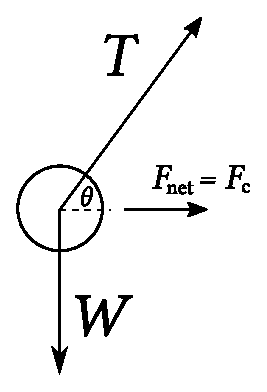
\includegraphics[width=1.8cm]{3.eps}}& $T\sin\theta = mg \text{~~~~;~~~~} T\cos\theta = ma = m(0.5g)$ \\
					& $\implies \tan\theta = \nicefrac{1}{0.5} = 2$ \\
					& $T = \left(\nicefrac{1}{\sin\theta}\right) mg = \left(\frac{2}{\sqrt{2^2 + 1^2}}\right)^{-1} mg = \doubleunderline{1.118mg}$
				\end{tabular}
			\end{center}
			\pagebreak[2]
		\item \solution{A}{Static Friction}
		
			This question is a bit tricky and debatable, it is more of trying to find out what the examiner wants, versus, what is actually the correct answer. 
			
			For a sphere to be able to roll, there must be static friction on the bottom on the sphere so that at that point, $v = 0$. The origin of this static friction is weight, because that is what provides for the energy for the ball to roll down a inclined plane. So it seems, it could be ``Static Friction" or ``Weight", it's not very clear cut. In fact, ``Static Friction" can only do negative work.
			
			The trick here now is that the word ``directly" was used. This suggests that the examiner is probably looking for ``Static Friction" as the answer, instead of ``Weight". 
		\vfill
		\item \solution{C}{$\displaystyle \frac{l}{3}$}
		
			\begin{minipage}[c]{4cm}
				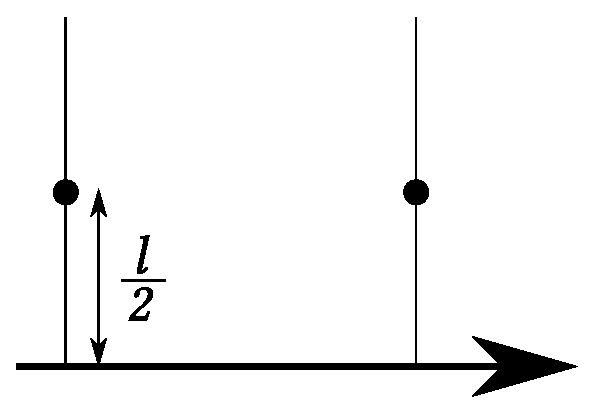
\includegraphics[width=3.5cm]{5.eps}
			\end{minipage}%		
			\begin{minipage}{\textwidth - 5cm}
				Assuming that the wire is of constant density $\sigma$, we take moments about the bottom wire:
				\begin{align*}
					\cancel{2}\times \cancel{l\sigma} \times \left(\frac{l}{\cancel{2}}\right) &= 3\cancel{l\sigma}x_{\text{cm}} \\
					x_{\text{cm}}&=\frac{1}{3}l
				\end{align*}
			\end{minipage}
		\vfill
		\item \calc \solution{C}{\SI{3.58}{\kilogram}}
		
			\begin{minipage}[c]{4.5cm}
				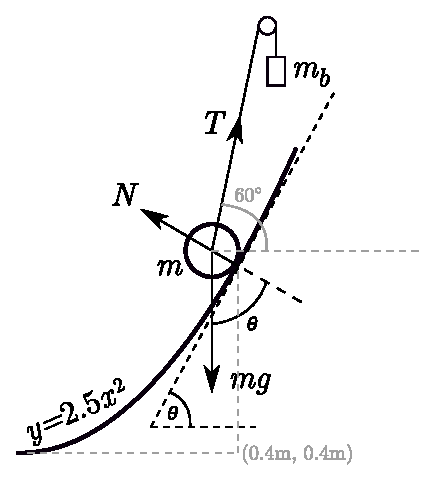
\includegraphics[width=4cm]{6.eps}
			\end{minipage}%	
			\setlength{\currentparskip}{\parskip}		% save the value
			\begin{minipage}{\textwidth - 6cm}
				\setlength{\parskip}{\currentparskip}	% restore the value
				We resolve all forces along the slope at $\left(\SI{0.4}{\meter}, \SI{0.4}{\meter}\right)$:
				\begin{gather*}
					T\cos\left(60\degree - \theta\right) = m_b \cancel{g}\cos\left(60\degree - \theta\right) = m\cancel{g}\sin\theta \\
					\implies m_b = m\frac{\sin\theta}{\cos\left(60\degree - \theta\right)}
				\end{gather*}
				We now differentiate $y=2.5x^2 \implies y' = 5x$ to obtain the gradient at $\left(\SI{0.4}{\meter}, \SI{0.4}{\meter}\right) = 5\times0.4 = 2$.
				
				Substitute $\theta = \arctan 2$, we obtain $m_b = \doubleunderline{\SI{3.58}{\kilogram}}$.
			\end{minipage}
		\vfill
		\item \solution{E}{$\displaystyle \frac{g}{4}$}
		
			Friction provides for the centripetal acceleration.		
			\begin{align*}
				\left(f=\mu_s N = \right) \mu_s \cancel{m}g &= \cancel{m}r\omega^2 \left(= F_c\right) \\
				a = r\omega^2 &= \mu_s g \\
				&= \doubleunderline{\frac{1}{4}g}
			\end{align*}
			% \pagebreak
		\item \solution{D}{$6$ Earth radii from surface of Earth}
			\begin{align*}
				a_c = G\frac{m_{\!_E}}{R^2} &= R\omega^2 \\ 
				R^3 &= G\frac{m_{\!_E}}{\omega^2} = G\frac{m_{\!_E}}{\left(\frac{2\pi}{T}\right)^{\!2}} \implies R = 6.6R_{\!_E} \approx 7 R_{\!_E}
			\end{align*}
			Since the question asks for height above Earth's surface, $\doubleunderline{R' \approx 6R_{\!_E}} $.
			\vfill
			\item \solution{B}{$\displaystyle \frac{2}{5} ma^2$}
			
			We know that an object's moment of inertia is given by $\displaystyle I = \int_{0}^{M} r^2 \dif m = \sum_{i}m_ir_i^2$. 
			
			Thus, the moment of inertia of the octant can be given by:
			\begin{equation*}
				I' = \frac{1}{8}\left(\frac{2}{5}\right)Ma^2 = \frac{1}{20}Ma^2 = \frac{1}{20}\left[8m\right]a^2 = \doubleunderline{\frac{2}{5} ma^2}
			\end{equation*}
			
			This makes sense intuitively too, the octant will be $\frac{1}{8}$ easier to spin, and then you convert $M$ to $m$, and you will obtain the same answer.
			\vfill
		\item \solution{E}{}
		
			As the object undergoes positive acceleration from rest, velocity $v$ becomes positive. Thus, the first part of the $s-t$ graph would be that of a positive quadratic curve. 
			
			Thereafter, the object undergoes motion with constant velocity. Thus, the second part of the $s-t$ graph would be that of a straight line with constant gradient $v$. 
			\vfill
		\item \solution{B}{\SI{1.76}{\second}}
		
			We take the constant velocity trailer as our frame of reference. Thus, the final velocities become:
			\vspace{-1em}
			\begin{equation*}
				v_t' = u_c' = 10-10 = \SI{0}{\meter\per\second} \text{~~~~and~~~~~}v_c' = 35-10 = \SI{25}{\meter\per\second}
			\end{equation*}
			Since the head of the car has to overtake the trailer and the car has to be one car-length ahead, the total relative displacement that the head of the car has to travel is:
			\begin{equation*}
				s_c' = 15.0 + 3.5 + 3.5 = \SI{22}{\meter}
			\end{equation*}
			Since the car undergoes uniform acceleration ($v-t$ graph is a straight line),
			\begin{align*}
				s &= \frac{1}{2} (u' + v') T \\
				22 &= \frac{1}{2} (25)T \implies T = \doubleunderline{\SI{1.76}{\second}}
			\end{align*}
		% \pagebreak
		\item \solution{A}{\SI{1121}{\newton}}
			% https://tex.stackexchange.com/a/122779
			\begin{equation*}
				\begin{cases}
					~600\sin 60 \degree + T\cos\theta &= 1600 \\
					~600\cos 60 \degree &= T\sin\theta 
				\end{cases} 
			\end{equation*}
			\vspace{-1.5em}
			\begin{align*}
				600\sin 60 \degree + \frac{600\cos 60 \degree}{\sin\theta} \cos\theta &= 1600 \\
				\implies \theta = 15.52 \degree \implies T = \doubleunderline{\SI{1121}{\newton}}
			\end{align*}
		%\vfill
		\item \solution{A}{\SI{30}{\second}}
			\vspace{-0.5cm}
			\begin{align*}
				v = u+at \implies 120 &= 70 + 6000t \\
				t &= \frac{1}{120}\SI{}{\hour} = \doubleunderline{\SI{30}{\second}}
			\end{align*}
		%\vfill
		\item \solution{E}{\SI{2.5}{\meter\per\second}}
			\begin{multicols}{2}
				\noindent
				\begin{align*}
					e = 0.5 &= \frac{v_2 - v_1}{u_1 - u_2} \\
					0.5\left(2 + 5\right) &= v_2 - v_1 \\
					v_2 &= v_1 + \frac{7}{2}
				\end{align*}
				\begin{gather*}
					m_1u_1 + m_2 u_2 = m_1v_1+m_2\left(v_1 + \frac{7}{2}\right) \\
					\implies v_1 = \SI{-1}{\meter\per\second} ~~\text{and}~~ v_2 =  \doubleunderline{\SI{2.5}{\meter\per\second}}
				\end{gather*}
			\end{multicols}
		%\vfill
		\item \calc \solution{D}{$\displaystyle F_0\left[T\left(1-\frac{1}{e}\right)-T\left(\frac{1}{e}\right)\right]$}
		
			\begin{equation*}
				\text{Let } x = \frac{t}{T} \implies \dod{x}{t} = \frac{1}{T} \implies \dif x = \frac{1}{T} \dif t
			\end{equation*}
			Given $t_0 = T$ : 
			\begin{align*}
				\int_{0}^{t_0} F_0 \left(\frac{t}{T}\right) e^{-\frac{t}{T}} dt &= T\int_{0}^{t_0} F_0 \left(\frac{t}{T}\right) e^{-\frac{t}{T}} \left(\frac{1}{T}\right) dt \\
				&= T F_0\int_{x\left(t=0\right) = 0}^{x\left(t=t_0\right) = 1} xe^{-x} \dif x \\
				&= T F_0 \left[1-(1+1)e^{-1}\right] \\
				&= TF_0 \left[1-\frac{2}{e}\right] &\equiv F_0\left[T\left(1-\frac{1}{e}\right)-T\left(\frac{1}{e}\right)\right]
			\end{align*}
		%\vfill
		\item \solution{E}{\SI{-0.33}{\meter\per\second\squared}}
			\begin{equation*}
				\frac{\Delta v}{\Delta t} = \frac{-6}{18} = \doubleunderline{\SI{-0.33}{\meter\per\second\squared}}
			\end{equation*}
		%\vfill
		\item \solution{C}{\SI{144}{\meter}}
			\begin{equation*}
				S = \text{area} = \frac{1}{2} \times 48 \times 6 = \doubleunderline{\SI{144}{\meter}}
			\end{equation*}
		
		\pagebreak
		\item \solution{C}{\SI{8.78}{\meter}}
			\begin{align*}
				\text{Using Conservation of Energy:} &&\frac{1}{2}\cancel{m}u^2 + \cancel{m}gh &= \frac{1}{2}\cancel{m}v^2 \\
				&&v &= \sqrt{2gh + u^2} 
			\end{align*}
			\vspace{-\parskip}
			In the $y$-direction:
			\vspace{-\parskip}
			\begin{align*}
				s &= ut+\frac{1}{2}at^2 \\
				10 &= v\sin 30\degree t + \frac{1}{2}gt^2 = \sqrt{2gh + u^2}\sin 30\degree t + \frac{1}{2}gt^2  \\
				t &= 1.002 \text{~~~~(reject the other negative value)}\\
				\implies d &= v\cos 30 \degree t = \doubleunderline{\SI{8.776}{\meter}}
			\end{align*}
		\vfill
		\item \solution{C}{\SI{25.5}{\meter}}
			\begin{align*}
				\text{All the GPE is converted to KE:}&& mgh &= \frac{1}{2} kx^2 \\
				&& \implies x &= 17.5 \implies l = 40-17.5 = \SI{25.5}{\meter}
			\end{align*}
		\vfill
		\item \solution{B}{\SI{13.6}{\meter}}
		
		Taking left as positive, applying conversation of momentum:
			\vspace*{-0.5em}
			\begin{align*}
				m_{\!_D}v_{\!_D} + m_{\!_B}v_{\!_B} &= 0 \text{~~~~~~~~~~~~~~~~~~~(relative to stationary shore)} \\
				v_{\!_D}&= -\frac{m_{\!_B}}{m_{\!_D}}v_{\!_B}
			\end{align*}
			\vspace{-1.5em}
			
			Integrating both sides:
			\vspace{-1em}
			\begin{align*}
				S_{\!_D}&= -\frac{m_{\!_B}}{m_{\!_D}}S_{\!_B} \\
				\left(\because S_{\!_D} = 8.0 + S_{\!_B}\right) ~~\therefore 8.0 + S_{\!_B} &= -\frac{m_{\!_B}}{m_{\!_D}}S_{\!_B} \\
				S_{\!_B} &= -\frac{8}{5} \\
				&\implies S_{\!_D} = 8.0 -\frac{8}{5} = 6.4 \\
				&\implies \text{Distance} =20-6.4 = \SI{13.6}{\meter}
			\end{align*}
			\textit{\small Refer to Dynamics Problem Set/Challenging Questions/Q1 for a similar question.}
		\vfill
		\item \solution{C}{\SI{2.000}{\second}} 
		
		$\omega$ is independent of amplitude.
		\pagebreak[4]
		\item \solution{E}{\SI{180}{\micro\meter}}
		
			There are more than one way of interpreting this question, so we are also not too sure how to go about doing this. In particular, the oscillation of the field may not be simple harmonic. 
			
			But, for the purpose of SJPO, it is \textit{often} correct to assume an oscillation to be simple harmonic. 
			
			Let $A_0$ be the amplitude of the oscillating electric field:
			\begin{align*}
				a = -\omega^2x \implies a_{\text{max}} &= -\omega^2 x_{\text{max}} \\
				\frac{qA_0}{m_e} &= -\omega^2 x_{\text{max}} \implies x_{\text{max}} = \SI{4.449e-5}{\meter} \\
				\implies S &= 4x_\text{max} = \SI{1.78e-4}{\meter} = \doubleunderline{\SI{180}{\micro\meter}}
			\end{align*}
			
		\item \solution{A}{\SI{0.038}{\femto\second}}
		
			Let $\sigma$ be the charge density of the ball, and $Q$ and $R$ be the total charge and radius of the ball. We take positive $r$ as outward from the centre. 
			
			To find the restoring force pulling on the electron after it passes the equilibrium point, we first consider the electric field:
			\vspace{-0.7em}
			\begin{equation*}
				E = k \frac{q_\text{below}}{r_{\text{below}}^2} = k \frac{\sigma \left(\frac{4}{3}\pi \cancelto{r}{r_\text{below}^3}\right)}{\cancel{r_{\text{below}}^2}} = k\sigma \frac{4}{3} \pi r_\text{below}
				\vspace{-0.7em}
			\end{equation*}
			Given $\displaystyle \sigma = \frac{Q}{\frac{4}{3}\pi R^3}$:
			\vspace{-1em}
			\begin{equation*}
				E = k \left(\frac{Q}{\cancel{\frac{4}{3} \pi} R^3}\right)\left(\cancel{\frac{4}{3} \pi} r_\text{below}\right) = \frac{kQ}{R^3}r_\text{below}
			\end{equation*}
			Since $F = qE$, we can obtain the acceleration $a$ of the electron at any position:
			\begin{align*}
				a &= \frac{qE}{m_e} = -\left(\frac{k|Qq|}{R^3 m_e}\right) r \left[\equiv -\omega^2 x\right] \implies \omega =\sqrt{\frac{k|Qq|}{R^3 m_e}} \\
				\implies \frac{1}{4} T &= \frac{2\pi}{4\omega} = \frac{\pi}{2\sqrt{\frac{k|Qq|}{R^3 m_e}}} = \doubleunderline{\SI{3.81e-17}{\second}}
			\end{align*}
			\textit{(Note that $k = \frac{1}{4\pi\varepsilon_0}$)}
		\pagebreak[4]
		\item \solution{C/D}{This is simple harmonic oscillator has two very different frequencies/This cannot even be a simple harmonic oscillator.}
			\begin{equation*}
				y = 2.0\cos\left(3.5t\right)\sin\left(3.7t\right) = \sin\left(7.2t\right)+\sin\left(0.2t\right)
			\end{equation*}
			Thus, the frequency of the 2 component waves are $\frac{7.2}{2\pi}$ and $\frac{0.2}{2\pi}$ respectively, with a ratio of $\frac{7.2}{0.2} = 36$.
			
			The first argument is that, as the ratio of the component waves is large enough, the motion of the oscillator will be such that it is sufficiently close to being simple harmonic that we may call it a ``simple harmonic oscillator", albeit with ``noise",  \doubleunderline{$\implies$ Option C}
			
			In fact, it probably is a simple harmonic oscillator oscillating around an equilibrium that is also undergoing simple harmonic motion.
			
			The counter argument is then that the defining equation of SHM is: 
			\begin{equation}
				F \propto -x \label{eqn:shm}
			\end{equation}
			Since we cannot write out an equation for $F$ that fulfils \eqref{eqn:shm} that involves the 2 component frequencies, it does not make sense to call it a simple harmonic oscillator. In fact, by including Option D, the examiner might be suggesting that the student think carefully about what constitutes a simple harmonic oscillator. \doubleunderline{$\implies$ Option D}
			
			Thus, we include here both arguments, and consequently both options, for the sake of discussion and completeness.
		%\pagebreak[2]
		\item \solution{C}{\SI{1.1}{\hertz}}
			\vspace{-0.5em}
			\begin{align*}
				y &= 3.0\cos\left(3.6t\right)\sin\left(3.6t\right) \\
				&= 1.5\sin\left(2\times 3.6t\right)  \\
				&= 1.5\sin \left(7.2t\right) \implies \omega = 7.2 \\
				f &= \frac{\omega}{2\pi} = \doubleunderline{\SI{1.14}{\hertz}}
			\end{align*}
		
		\item \solution{E}{\SI{4.2}{\meter}}
			\begin{equation*}
				1.5 = \frac{2\pi}{\lambda} \implies \lambda = \doubleunderline{\SI{4.19}{\meter}}
			\end{equation*}
			
		\item \solution{B}{negative-$x$ direction}
		
			For a wave with equation $y\left(x,t\right) = A\cos\left(kx-\omega t\right)$, the phase velocity $v_p$ is given by:
			\begin{equation*}
				v_p = \frac{\omega}{k} = \frac{-3.6}{1.5} = -2.4 \implies \text{negative-$x$ direction}
			\end{equation*}
		
		\item \solution{A}{This wave has two very similar frequencies. $\left(\text{ratio} < 2\right)$} 
		
			This resultant wave is an example of beats. 
		
		\item \solution{B}{The wave speed is \SI{2.4}{\meter\per\second}}
		
			\begin{minipage}[c]{5.5cm}
				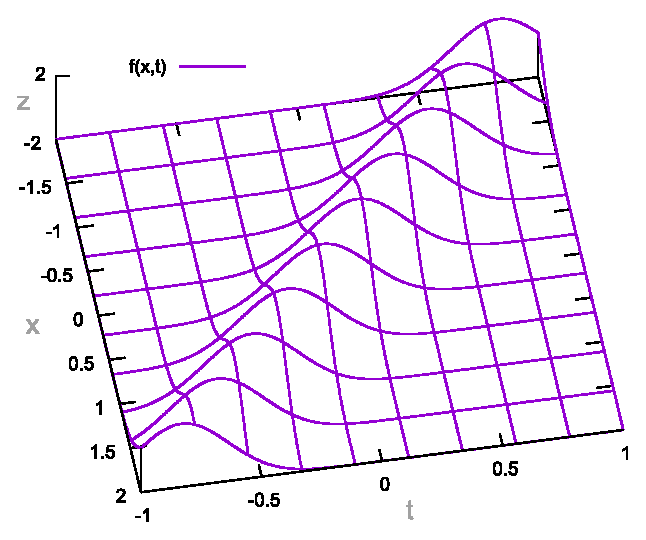
\includegraphics[width=5cm]{29.eps}
			\end{minipage}%	
			\setlength{\currentparskip}{\parskip}		% save the value
			\begin{minipage}{\textwidth - 7cm}
				\setlength{\parskip}{\currentparskip}	% restore the value
				From the plot, we see that this is a pulse wave\footnote{With some analysis of the given plot in the paper, we can also deduce the wave only has an amplitude of 2 at one point in space given a point in time, and is thus a pulse.}.
				
				Since $y = 2.0e^{-\left(1.5x+3.6t\right)^2}$, we examine the speed that the peak of the pulse is travelling. At maximum amplitude:
				\begin{align*}
					e^{-\left(1.5x+3.6t\right)^2} &= 1 \\
					\implies -\left(1.5x+3.6t\right)^2 &= 0 \\
					\implies 1.5x+3.6t &= 0 \\
					x &= \frac{-3.6}{1.5}t \\
					\implies \dod{x}{t} &= \SI{2.4}{\meter\per\second}
				\end{align*}
			\end{minipage}
		
		\item \solution{C}{\SI{0.85}{\meter}}
		
			\begin{minipage}[c]{4.5cm}
				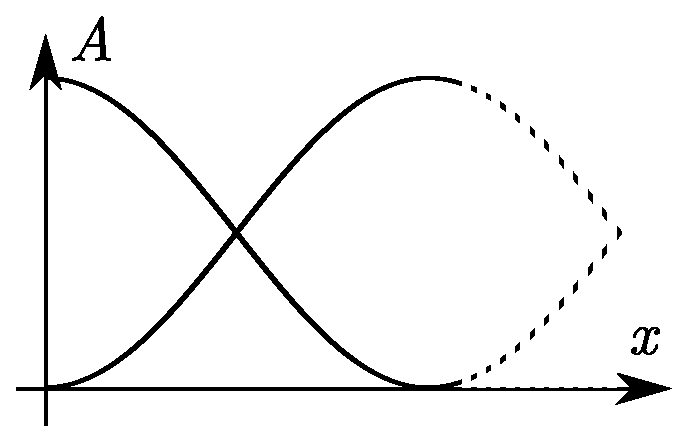
\includegraphics[width=4cm]{30.eps}
			\end{minipage}%	
			\setlength{\currentparskip}{\parskip}		% save the value
			\begin{minipage}{\textwidth - 6cm}
				\setlength{\parskip}{\currentparskip}	% restore the value
				\begin{align*}
					\lambda &= \frac{v}{f} = vT = \left(53\times 10^{-2}\right)\left(6.4\right) \\
					\text{nearest node~} = \frac{1}{4} \lambda &= \frac{1}{4}\left(53\times 10^{-2}\right)\left(6.4\right) = \doubleunderline{\SI{0.848}{\meter}}
				\end{align*}
			\end{minipage}
		
		\item \solution{B}{moves in a parabolic trajectory and hits the second plate}
		
			This is a simple question involving energy and 2D-Kinematics. For the purposes of this question, we can safely ignore the effects of gravity et al., and simply consider that the electron has total energy $\SI{1.5}{\electronvolt} > \SI{1}{\electronvolt}$ needed to reach the second plate.
			
			As the force only exists in the direction perpendicular to the plates, the electron undergoes parabolic motion and hits the second plate.
			
			\begin{center}
				\hdashrule{0.75\textwidth}{0.1mm}{1pt}
			\end{center}
			{
				\setlength{\parskip}{0.5\parskip}
				\footnotesize 
				Actually, for the curious, we can do a back-of-the-envelope calculation of the energies involved:
				\begin{equation*}
					E = \SI{1.5}{\electronvolt} = G\frac{Mm_{\text{e}}}{r} + qV = \text{GPE} + \SI{1}{\electronvolt}
				\end{equation*}
				For the electron to not hit the second plate,
				\begin{equation*}
					\SI{0.5}{\electronvolt} < G\frac{Mm_{\text{e}}}{r} \implies \frac{M}{r} > \frac{10^{-17}}{10^{-11} \times 10^{-31}}  = 10^{25}
				\end{equation*}			
				which is ridiculous, considering that even if we put the plates on the surface of the Sun, $\frac{M}{r} = 10^{24} < 10^{25}$, the electron won't hit the second plate.  
				
				Furthermore, the question does not even state the direction of gravity.
				
				Thus, we can safely ignore the effects of gravity, and simply consider the electric potential energy involved. 
			}
			%\begin{center}
			%	\hdashrule{0.75\textwidth}{0.1mm}{1pt}
			%\end{center}
		
		\item \solution{E}{\SI{1.6e-26}{\newton} downwards}
		
			The force on the proton due to the downward electric field is downwards, thus:
			\begin{equation*}
				\sum F = mg + qE = \doubleunderline{\SI{1.64e-26}{\newton}}
			\end{equation*}
		
		\item \solution{C}{The mass of $P$ is less than that of $Q$}
			
			The force experienced by both charges is same. At equilibrium,
			\begin{align*}
				\text{Electric Potential Energy} &= \text{Gravitational Potential Energy} \\
				\because \text{EPE is equal~} \implies m_p \cancel{g} h_p &= m_q \cancel{g} h_q \\
				m_p &= \frac{h_q}{h_p} m_q \\
				\because h_q < h_p &\implies \doubleunderline{m_p < m_q}
			\end{align*}
			
			Alternatively, we may realize that the vertical line is the centre of mass of the system. 
		
		\item \solution{A}{\SI{2.3e-10}{\newton} upwards}
		
			\begin{minipage}[c]{3.5cm}
				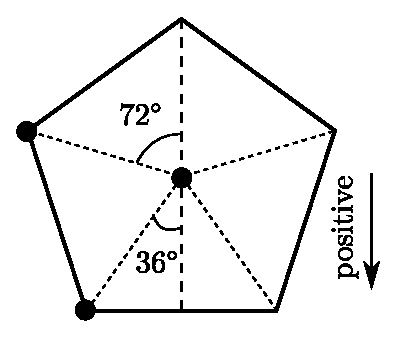
\includegraphics[width=3.5cm]{34.eps}
			\end{minipage}%	
			\setlength{\currentparskip}{\parskip}		% save the value
			\begin{minipage}{\textwidth - 5cm}
				\setlength{\parskip}{\currentparskip}	% restore the value
				\begin{align*}
					F_i &= k \frac{q^2}{r^2} \\
					\sum_i F_i &= \left(F_i\cos 72\degree\right) \times 2 - \left(F_i\cos 36\degree\right) \times 2 \\
					&= 2F_i \left(\cos 72 \degree - \cos 36\degree\right) \\
					&= \doubleunderline{\SI{-2.31e-10}{\newton}}
				\end{align*}
			\end{minipage}
		
		\item \solution{D}{may be calculated as 5 times the energy stored in a system of two point charges}
			
			The electric potential energy of a system may be calculated as the sum of all the electric potential energies, mathematically:
			\begin{equation*}
				E = \sum_{i, j} \frac{kq_iq_j}{r}
			\end{equation*}
			Since we are only concerned with the sixth proton, the electric potential energy is:
			\begin{equation*}
			E = \sum_{i} \frac{kq_6q_j}{r}
			\end{equation*}
			Since the charges are identical, and the placement of the protons are symmetrical, the EPE between every other proton and this sixth proton would be identical. 
			
			Thus, since there are 5 pairs of charges in the system, the electric potential energy associated with the sixth proton may simply be calculated as 5 times the energy stored in a system of two point charges.
			
		\item \solution{B}{\SI{1.5e-12}{\meter}}
		
			$\sum P = 0$, thus the closest the protons can get is when all the Kinetic Energy is converted into Electric Potential Energy.
			\begin{align*}
				2\times \frac{1}{2}mu^2 &= k\frac{q^2}{r} \\
				r &= \frac{kq^2}{mu^2} = \doubleunderline{\SI{1.53e-12}{\meter}}
			\end{align*}
			
		\item \solution{B}{\SI{1.5e-12}{\meter}}
		
			The fastest way to do this question is to do a change in perspective --- by considering a moving frame of reference that moves at $v=\SI{3e5}{\meter\per\second}$. Since all laws of Physics hold in an inertial frame, we realize that this situation is same as that in Q36, yielding the same answer \doubleunderline{\SI{1.53e-12}{\meter}}.
			
			Alternatively, since $\sum p \neq 0$, the protons are the closest when $v_1 = v_2$:
			\begin{equation}
				mu = mv_1+mv_2 \implies mu = m \left(2v_1\right) \implies v_1 = v_2 = \frac{1}{2} u
			\end{equation}
			We now consider the energies:
			\begin{align*}
				\text{KE}_i &= \text{EPE} + \text{KE}_{\!f} \\
				\frac{1}{2} mu^2 &= \frac{kq^2}{r} + \cancel{\frac{1}{2}}m\left(\frac{1}{2}u\right)^2 \times \cancel{2} \\
				m\left(\frac{1}{2}u^2-\frac{1}{4}u^2\right) &= \frac{kq^2}{r} \\
				\frac{1}{4}mu^2 &= \frac{kq^2}{r} \implies r = \frac{kq^2}{\frac{1}{4}mu^2} = \doubleunderline{\SI{1.53e-12}{\meter}}
			\end{align*}
			
		\item \solution{C}{\SI{10}{\micro\meter}} \textit{\small solution provided by Theodore}
		
			\begin{minipage}[c]{4cm}
				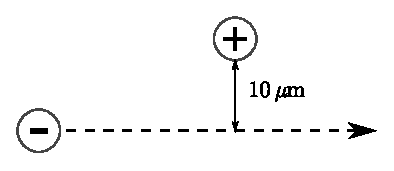
\includegraphics[width=3.5cm]{38.eps}
			\end{minipage}%	
			\setlength{\currentparskip}{\parskip}		% save the value
			\begin{minipage}{\textwidth - 5.1cm}
				\setlength{\parskip}{\currentparskip}	% restore the value
				Assume the proton is always stationary; Without electrostatic, the electron misses by \SI{10}{\micro\meter}
				
				$\implies$ Impact parameter $b$ is \SI{10}{\micro\meter}.
				\begin{align*}
					\text{angular momentum } J &= m_e u b \\
					 &= m_e\left(3\times 10^6\right)\left(3\times10^{-6}\right)
				\end{align*}
			\end{minipage}
		
			Now, we examine the situation with electrostatic force. Electrostatic force is a central force.  We can therefore say that:
			\begin{align}
				\text{Tangential KE} &= \frac{1}{2}mr^2\dot{\theta}^2 = \frac{J^2}{2mr^2} \\
				\text{i.e. ~} V_{\text{eff}} &= \frac{J^2}{2mr^2} - \frac{q^2}{4\pi\varepsilon_0 d}
			\end{align}
			At closest approach, $\dot{r} = 0$:
			\begin{align*}
				E &= \frac{1}{2} m_eu^2 \text{~~~~(assume potential at $\infty = 0$)} \\
				\frac{1}{2}m_eu^2 &= \frac{m_e^{\cancel{2}}u^2b^2}{2\cancel{m_e}d^2} - \frac{q^2}{4\pi\varepsilon_0 d}\\
				m_e u^2d^2 + \frac{q^2}{2\pi \varepsilon_0}d - m_eu^2b^2 &=	0 \\
				d^2 + \frac{q^2}{2\pi\varepsilon_0u^2} - b^2 &= 0
			\end{align*}
			Let $\beta = 2\pi\varepsilon_0u^2$, rearranging the previous equation:
			\begin{align*}
				d&= \frac{-\beta+\sqrt{\beta^2+4b^2}}{2} \\
				\because \beta &= \frac{\left(1.6\times 10^{-19}\right)^2}{2\pi\varepsilon_0\left(3\times10^6\right)^2} \\
				&= 5.615 \times 10^{-11} \ll 10\times 10^{-6} \implies \therefore  d \approx b \implies \text{\doubleunderline{Option C}}
			\end{align*}
		\vfill
		\item \solution{A}{right}
			\begin{center}
				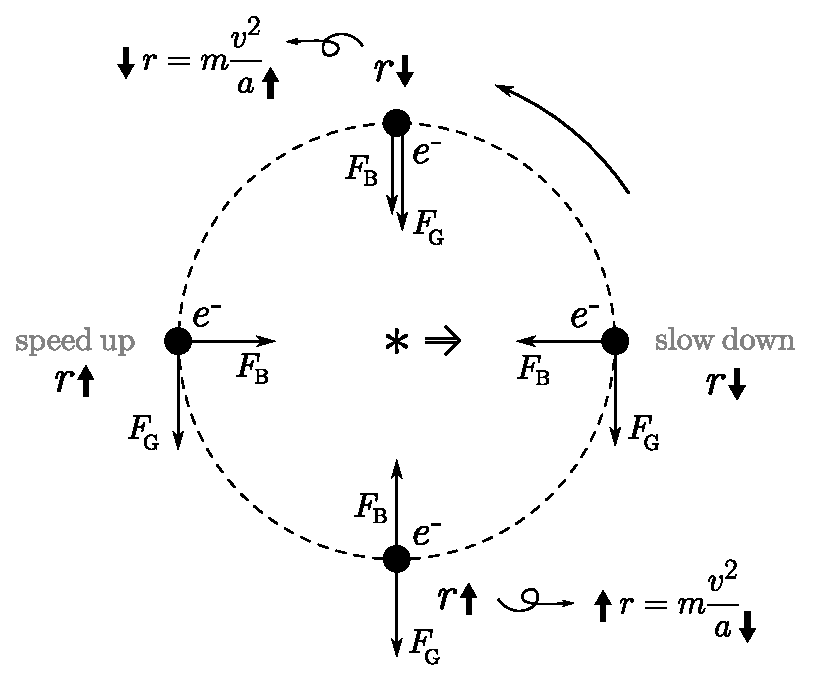
\includegraphics[width=11cm]{39.eps}
			\end{center}
		\vfill
		\pagebreak
		\item \solution{D}{\SI{0.071}{\milli\meter}}
		
			\begin{minipage}[c]{5cm}
				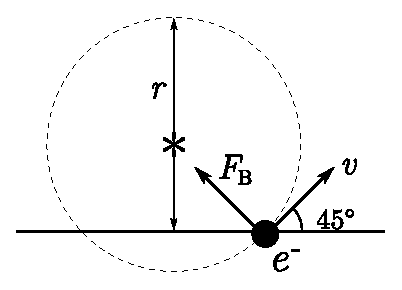
\includegraphics[width=4.5cm]{40.eps}
			\end{minipage}%	
			\setlength{\currentparskip}{\parskip}		% save the value
			\begin{minipage}{\textwidth - 7cm}
				\setlength{\parskip}{\currentparskip}	% restore the value
				\noindent
				\begin{align*}
					|F| = |qvB| &= m\frac{v^2}{r} \\
					r &= m\frac{v^2}{|qvB|} = \frac{mv}{|qB|} = \frac{\sqrt{E_k\left(2m\right)}}{|qB|} \\
					\text{Furthest} &= r + r\sin 45\degree \\
					&= r\left(1+\sin 45 \degree \right) \\ 					
					&= \frac{\sqrt{E_k\left(2m\right)}}{|qB|}\left(1+\sin 45 \degree \right) \\
					&= \SI{0.0705}{\milli\meter}
				\end{align*}
			\end{minipage}
		
		\item \solution{E}{\SI{80}{\ohm}}
		
			\begin{minipage}[c]{4.5cm}
				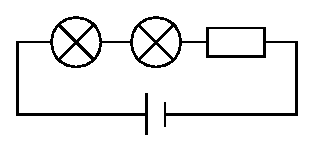
\includegraphics[width=4cm]{41.eps}
			\end{minipage}%	
			\setlength{\currentparskip}{\parskip}		% save the value
			\begin{minipage}{\textwidth - 6.5cm}
				\setlength{\parskip}{\currentparskip}	% restore the value
				\noindent
				The current is the same throughout the entire circuit. Thus, $I_\text{LED} = I = \SI{20e-3}{\ampere}$
				\begin{equation*}
					I_\text{LED} = \frac{V_\text{LED}-V_\text{th}}{R_\text{LED}} \implies V_\text{LED} = I_\text{LED}R_\text{LED} + V_\text{th}
				\end{equation*}
			\end{minipage}
			\begin{align*}
				V &= \sum I\!R \\
				6.0 &= 2V_\text{LED} + I_\text{LED}R \\[0.3em]
				&= 2\left[I_\text{LED}R_\text{LED} + V_\text{th}\right] + I_\text{LED}R \\[0.3em]
				R &= \frac{6.0 - 2\left[I_\text{LED}R_\text{LED} + V_\text{th}\right]}{I_\text{LED}} = \frac{6.0 - 2\left[\left(20\times 10^{-3}\right)\left(10\right) + 2\right]}{20\times 10^{-3}} = \doubleunderline{\SI{80}{\ohm}}
			\end{align*}
			
		\item \solution{D}{\SI{0.10}{\ampere}}
			\begin{equation*}
				P = IV \implies I = \frac{P}{V} = \frac{12}{\nicefrac{240}{2}} = \doubleunderline{\SI{0.10}{\ampere}}
			\end{equation*}
			
		\item \solution{D}{\SI{9.10e-6}{\ohm\meter}}
		
			For a battery with internal resistance, the terminal voltage of the battery is given by:
			\begin{equation}
				V_\text{batt} = \varepsilon - I\!R
			\end{equation}
			The potential difference across the wire is equal to the terminal voltage of the battery:
			\begin{align*}
				 R_{\text{wire}} = \frac{V_\text{batt}}{I} = \frac{\varepsilon - I\!R}{I} &= \rho \frac{l}{A} \\[0.5em]
				\rho &= \frac{A\left(\varepsilon-I\!R\right)}{Il} \\
				&=\frac{\pi r^2\left(\varepsilon-I\!R\right)}{Il} = \doubleunderline{\SI{9.12e-6}{\ohm\meter}}
			\end{align*}
			
		\item \solution{C}{\SI{1.0}{\ampere}} \textit{Solution made with input from Theodore}
		
			%At first look, this might look like an RLC-circuit question. However, it turns out, we don't actually require any specific RLC-circuit knowledge. However, we must still know how to calculate the impedance of each individual component. 
			
			When dealing with AC, we use complex impedances. \textit{(Note that $j = \sqrt{-1}$)}
			
			For the capacitor:
			\begin{equation*}
				\frac{\tilde{V}}{\frac{1}{j \omega C}} = \tilde{V}j \omega C = \tilde{I}\\
			\end{equation*}
			Taking the amplitude,
			\begin{equation}
				I = V\!\omega C \implies \omega C = \frac{I}{V} \implies \frac{1}{\omega C} = \frac{V}{I} = 1 \label{eqn:44:capacitor}
			\end{equation}
			Similarly, for the inductor:
			\begin{equation}
				\frac{\tilde{V}}{\tilde{I}} = j\omega L  \implies \omega L = \frac{V}{I} = 1
			\end{equation}
			Again, similarly, for the resistor:
			\begin{equation}
				\frac{\tilde{V}}{\tilde{I}} = R  \implies \frac{V}{I} = R = 1
			\end{equation}
			Thus, we find that for all 3 components:
			\begin{equation*}
				\frac{1}{\omega C} = R = \omega L = 1
			\end{equation*}
			When all are in series, we can find the effective impedance by adding up the complex impedances:
			\begin{equation*}
				\tilde{I} = \frac{\tilde{V}}{R + j\omega L + \frac{1}{j\omega C} } = \frac{\tilde{V}}{R + j\left(\omega L - \frac{1}{\omega C}\right)} = \frac{\tilde{V}}{R} = \doubleunderline{\SI{1.0}{\ampere}}
			\end{equation*}
			
			\textit{\textbf{Note:} resonance occurs, impedance purely resistive.}
				
			\textit{The inductor and capacitor will lag and lead the resistor by the same phase difference, and since they have the same magnitude, it will cancel out nicely.}
			
			%Given impedance $Z = \nicefrac{V}{I}$, we find that the impedance $Z_i$ of all the components are:
			%\begin{equation*}
			%	Z_{\!R} = Z_C = Z_{\!L} = \frac{1.0}{1.0} = \SI{1.0}{\ohm}
			%\end{equation*}
			%When connected in series:
			%\begin{align*}
			%	I_\text{resultant} = \frac{V}{Z_{\text{resultant}}} = 					\frac{\cancel{1.0}}{\cancel{1.0}\times 3} = \doubleunderline{\nicefrac{1}{3}\SI{}{\ampere}}
			%\end{align*}
		
		%\vfill
		\pagebreak
		\item \solution{B/D/E}{[\SI{1}{\ampere},\SI{1}{\ampere},\SI{1}{\ampere}] / [\SI{1}{\ampere},\SI{1}{\ampere},\SI{2}{\ampere}] / [\SI{2}{\ampere},\SI{1}{\ampere}, it doesn't make sense to talk about the current]}
			
			\textbf{Disclaimer: We are not sure about this question. This question was very weirdly phrased.}
			
			First, we consider that current cannot be negative, but can have a direction. Looking at any single component (including a battery), we realize that there is \SI{1}{\ampere} of current flowing into the component, and \SI{1}{\ampere} of current flowing out of the component. In total, there will be \SI{2}{\ampere} of current flowing through the component. This is more so because of the way the question phrased $\implies$ \doubleunderline{Option D}
			
			However, if the question is simply testing about the conservation of charge, then the answer is simply that there is only \SI{1}{\ampere} of charge going around. $\implies$ \doubleunderline{Option B}
			
			Let's now then consider the mechanics of a battery. In a classical cell battery, there is an electrolyte, a cathode and an anode. Reduction happens at the cathode, while oxidation happens at the cathode. This results in a flow of charges between the nodes in the form of ions, which produces a current through the wire that connects the anode and cathode. Thus, from this perspective, there is no current through the surface of the battery, only through the inside of the battery, $\implies$ \doubleunderline{Option E}
		
		%\vfill
		\item \solution{C}{$O>N=S>P$}
		
			\begin{minipage}[c]{2.5cm}
				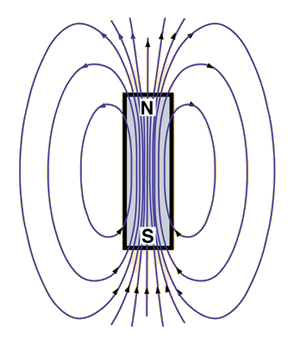
\includegraphics{46.png}
			\end{minipage}%	
			\setlength{\currentparskip}{\parskip}		% save the value
			\begin{minipage}{\textwidth - 3.6cm}
				\setlength{\parskip}{\currentparskip}	% restore the value
				\noindent
				$O$ should be have the strongest magnetic field since it is the centre of the magnet. As we move closer to the north and south pole of the magnet, the magnetic field lines will start to diverge, thus, $O > \left(N = S\right)$. Outside the magnet, the field lines diverge even more, thus $O > \left(N = S\right) > \left(P = Q\right)$. $R$ would have the weakest magnetic field as it is at the side of the magnet.
			\end{minipage}
		%\vfill
		%\pagebreak
		\item \solution{E}{\SI{160}{\kelvin}}
		
			\textit{Disclaimer: The answer obtained isn't close enough to \SI{160}{\kelvin} for me to be comfortable with it, so please take this solution with a pinch of salt.}
			\begin{align*}
				COP_{\text{heating}} = \frac{Q_C + W}{W} = \frac{kA \od{T}{x} + \frac{V^2}{R}}{\frac{V^2}{R}} &= \frac{T_\text{hot}}{\Delta T} \\
				kA \frac{\Delta T}{x} + \frac{V^2}{R} &= \frac{T_\text{hot}}{\Delta T} \left(\frac{V^2}{R}\right) \\
				\left(\frac{KA}{x}\right) \Delta T^2 + \left(\frac{V^2}{R}\right) \Delta T - \frac{T_\text{hot}V^2}{R} &= 0
			\end{align*}
			Rejecting the negative root, we obtain:
			\begin{equation*}
				\Delta T = \SI{150.9}{\kelvin} \implies \doubleunderline{\SI{160}{\kelvin}}
			\end{equation*}
		\item \solution{A}{added to the system minus the work done by the system}
			\begin{equation}
				\Delta U = Q + W_\text{on}
			\end{equation}
		\item \solution{E}{(i) and (ii)}
		
			\begin{minipage}[c]{4.5cm}
				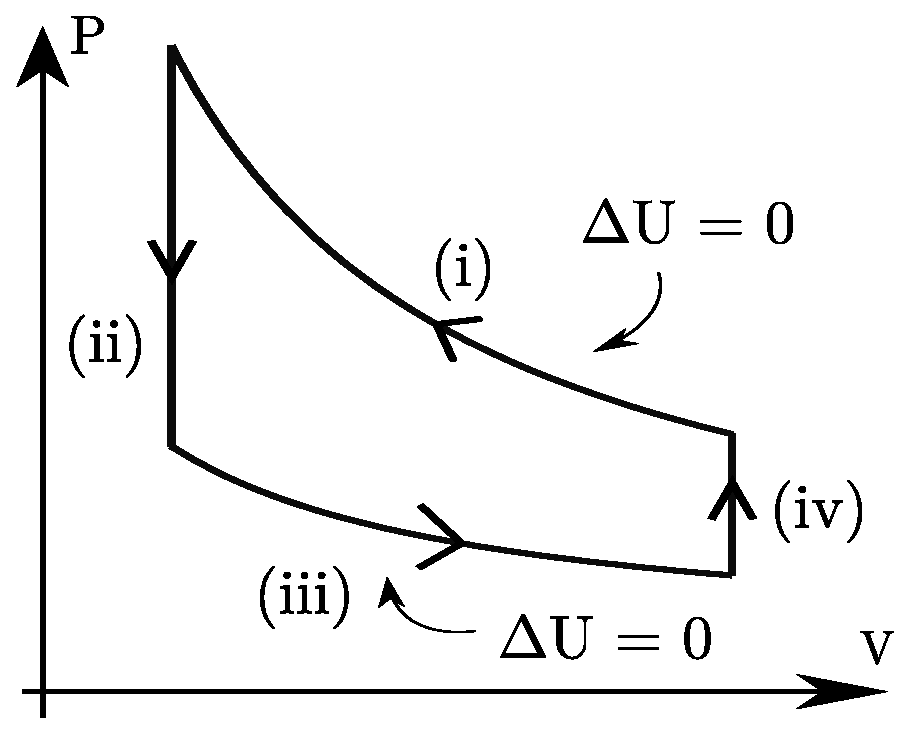
\includegraphics[width=4cm]{49.eps}
			\end{minipage}%	
			\setlength{\currentparskip}{\parskip}		% save the value
			\begin{minipage}{\textwidth - 5.6cm}
				\setlength{\parskip}{\currentparskip}	% restore the value
				\noindent
				Since this is a refrigerator, the gas cycle runs in the opposite direction of a Stirling engine.
				\begin{enumerate}[label={(\roman*)}]
					\item $\Delta U = 0$, $W_\text{on} > 0$, $\boxed{Q<0}$
					\item $\Delta U < 0$, $W_\text{on} = 0$, $\boxed{Q<0}$
					\item $\Delta U = 0$, $W_\text{on} < 0$, $\boxed{Q>0}$
					\item $\Delta U > 0$, $W_\text{on} = 0$, $\boxed{Q>0}$
				\end{enumerate}
				$\implies$ \doubleunderline{(i) and (ii)}
			\end{minipage}
		\item \solution{E}{Any of them}
		\vspace{0.5em}
			\begin{center}
				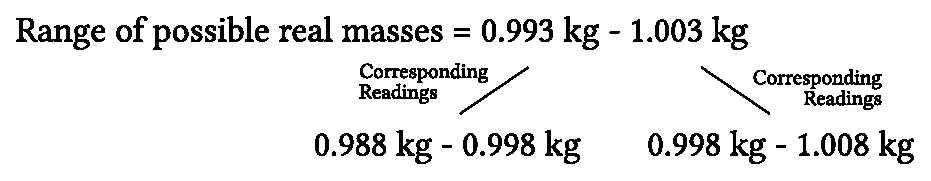
\includegraphics[width=0.7\textwidth]{50.eps}
			\end{center}
	\end{enumerate}
\end{document}